\chapter{Deterministic Model of Reproduction and Selection}
\ifpdf
    \graphicspath{{DeterministicModelofReproductionandSelection/Chapter2Figs/PNG/}{DeterministicModelofReproductionandSelection/Chapter2Figs/PDF/}{DeterministicModelofReproductionandSelection/Chapter2Figs/}}
\else
    \graphicspath{{DeterministicModelofReproductionandSelection/Chapter2Figs/EPS/}{DeterministicModelofReproductionandSelection/Chapter2Figs/}}
\fi
By determinism we means that given some conditions the final result is always  the same. For example if you know the initial frequencies and the rates of birth and death of two interacting species and measure  the frequencies at a certain time, this process is deterministic if every time  you set the same initial frequencies, you get the same final conditions at the same times. Deterministic population growth models are useful from understanding  the dynamic processes of growing and in predicting population frequencies and steady states. These deterministic models are divided in two types: discrete and continuos. This chapter gives some basic concepts of these two types that will be used for the development of this work. Furthermore in the last part of this chapter a continuos model of natural selection will be explained. 
\section{Discrete Model}
In discrete models of population growth the number $N$ of individuals increases with each time step $\Delta t$. The population at time $t+\tau$ is a recurrence function of the present generation at time $t$ and past populations, 
\begin{equation}
N_{t+\Delta t}=f(N_{t},N_{t-\Delta t}, ......, N_{0}),
\end{equation}
but usually it is just a function of the present population
\begin{equation}
N_{t+\Delta t}=f(N_{t}).
\end{equation} 
Given the initial conditions, the recurrence relation is solved if  it is possible to write $N_{n\Delta t }$ in terms of the initial conditions, $n$ and $\Delta t$. This allows us to know the state of the $n$ generation without using the recursion equation. 

Most of the recurrence relations have no solution, but even then, they  allow us to know about the properties of population dynamics, such as the existence of steady states. Due to this fact, they are essential for the algorithms in computational simulations of biological systems, as for example, the Fibonacci sequence for modeling rabbit population growth and plant patterning.

  
Now one of the most popular examples of discrete processes in literature will be shown. Suppose that at certain average period of time an individual divides; for example consider a cell and its offsprings that divide into  $r$ cells each time $\tau$. The  equation of this process is
\begin{equation}
N_{t+\tau}=rN_{t},
\end{equation} 
this is a recurrence equation, and the solution in terms of the initial condition $x_{0}$ after $n$ periods of time is
\begin{equation}
N_{n\tau}=N_{0}r^{n\tau}.
\end{equation}
The recurrence relation can be transformed to 
\begin{equation}
N_{t+\tau}-N_{t}=(r-1)N_{t},
\end{equation}
that is a difference equation of first order. 
For long times and taking $\tau=1$, this discrete equation can be transformed into a differential equation in time. 
\section{Continuous Model}
%Continuous model are good for population dynamics after times much larger than the time step of reproduction.
The most simple system in continuous growth is the single species model of birth. Where the per capita rate of change in population is due to the reproductive contribution $r$ of each individual,
\begin{equation}
\frac{dN(t)}{dt}=rN(t),
\end{equation} 
but this is for growth in a perfect environment. In a more realistic situation, without considering ecological interactions, there are death rate $d$ and migration $m$. Then the rate of change in the population would be 
\begin{equation}
\frac{dN(t)}{dt}=rN(t)-dN(t)-mN(t).
\end{equation}
 The solution of this equation is
 \begin{equation}
 N(t)=N_{0}e^{(r-d-m)t},
 \end{equation}
 where if $r-d-m$ is positive the population will growth and if $r-d-m$ it will decrease.
 
 Now let us see a continuous model of natural selection, where we have a population of constant size $N$ and two or more species competing. The constant size condition will generate selection and in a realistic situation it can be set up to maintain the population  at its maximum carrier capacity.
 
 Suppose we have two organisms $A$ and $B$ competing, with fitnesses $f_{A}$ and $f_{B}$ and frequencies $x_A$ and $x_B$ respectively. Because of the constant size $x_A+x_B=N$, there is a rate of death $\phi$ common to the two populations of organisms that keeps this condition. The differential equations for these two types are
 \begin{equation}
 \frac{dx_A}{dt} =f_A x_{A} - \phi,
 \end{equation}  
  \begin{equation}
 \frac{dx_B}{dt} =f_B x_{B} - \phi.
 \end{equation}  
 Solving these two equations for $\phi$
 \begin{equation}
 \phi = \frac{x_{A}f_{A}+x_{B}f_{B}}{N},
 \end{equation}
 and replacing $\phi$ in the equation for $x_{A}$, we obtain the differential equation for it
 \begin{equation}\label{3.12}
\frac{dx_{A}}{dt}=x_{A}(1-\frac{x_{A}}{N})(f_{A}-f_{B}).
 \end{equation} 
Its solution is 
\begin{equation}
x_{A}(t)=\frac{x_{A0}e^{(f_{A}-f_{B})t}}{1-\frac{x_{A0}}{N}+\frac{x_{A0}}{N}e^{(f_{A}-f_{B})t}}.
\end{equation}  
In these two equations it can be seen that the dominance of $A$ depends only on the fact that its fitness is larger than the fitness of $B$  (Figure \ref{Fig3.1}), and the time of fixation will be shorter if the initial population increases Figure (3.2). It can be seen also that the equilibrium points are the points of dominance. 
\begin{figure}[H]
  \begin{center}
    \leavevmode
    \ifpdf
      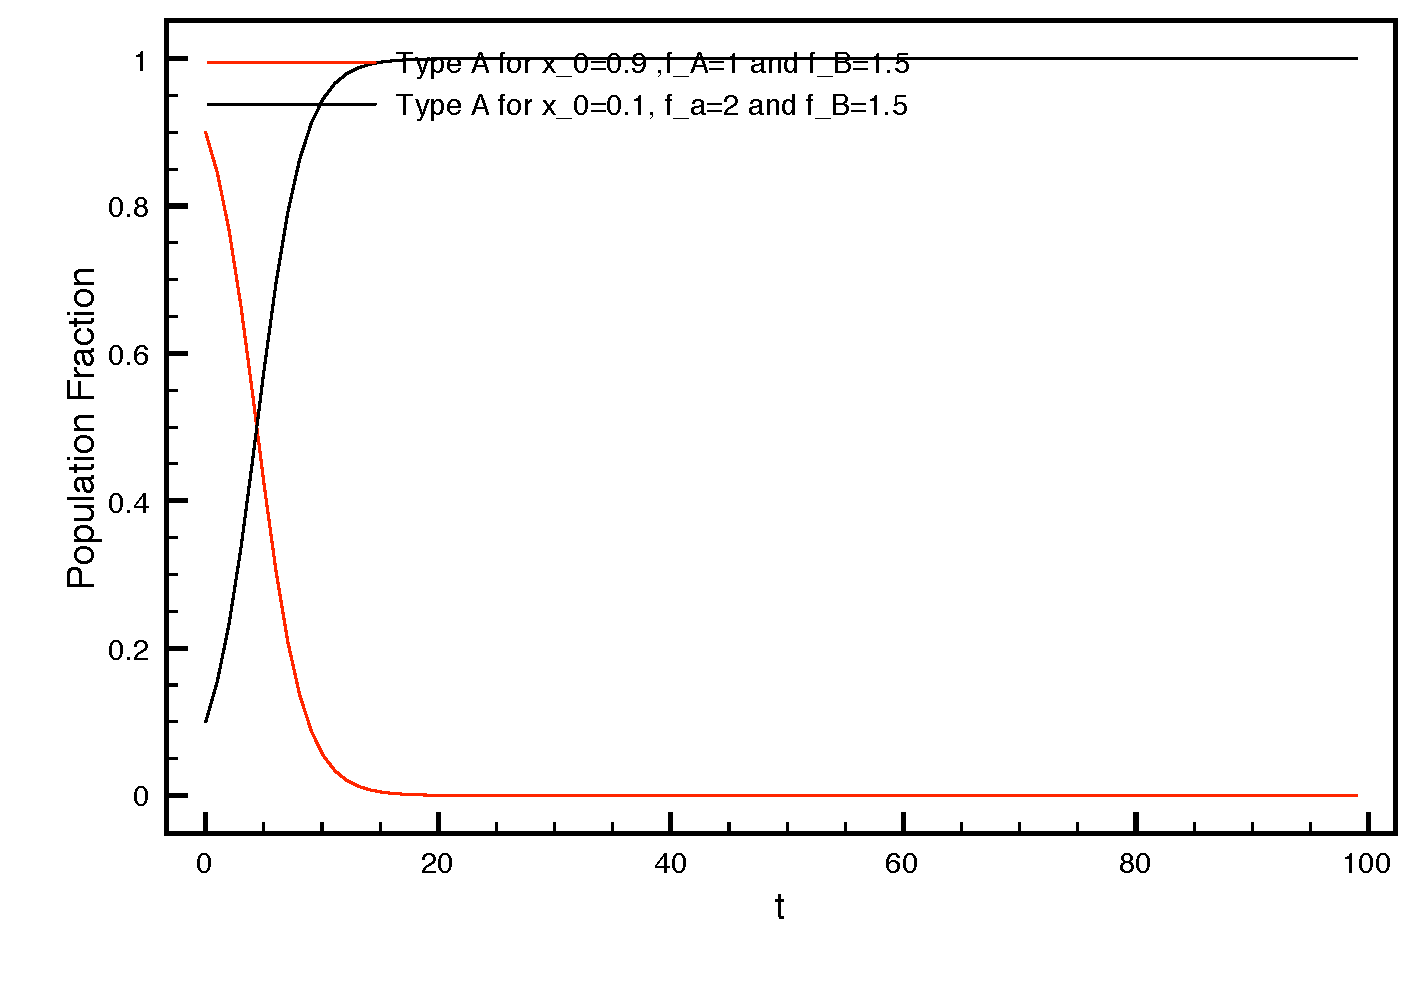
\includegraphics[width=7cm,height=7cm]{DeterministicSelection.pdf}
    \else
      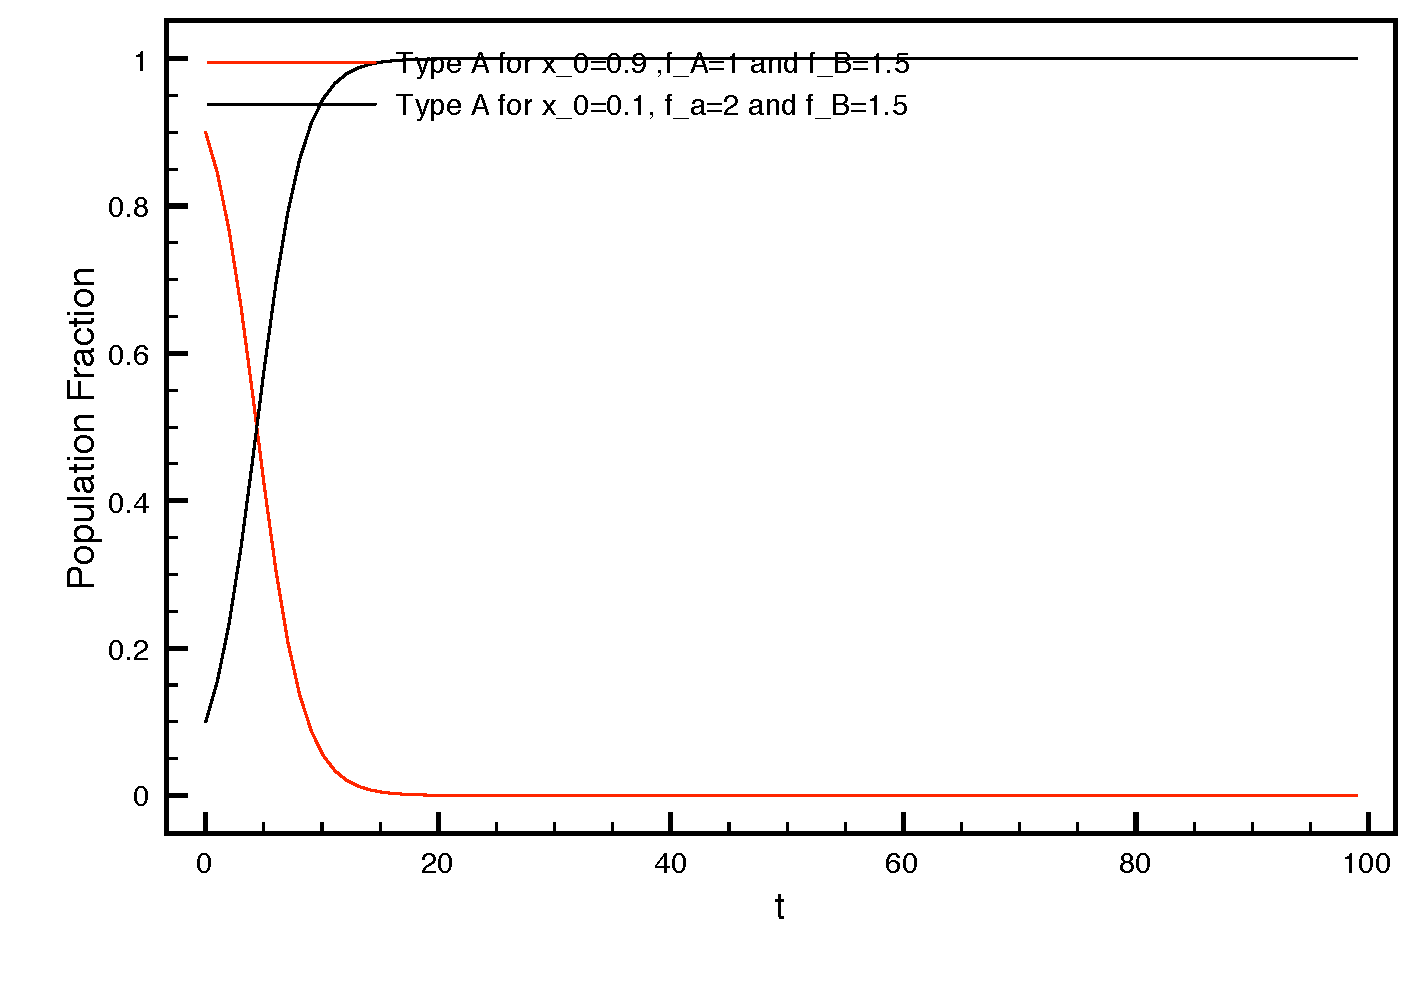
\includegraphics[width=7cm, height=7cm]{DeterministicSelection.pdf}
    \fi
    \caption{Fraction of $x_{A}$ for two different conditions of initial population and fitness.}
    \label{Fig3.1}
  \end{center}
  \end{figure}
  
\begin{figure}[H]
  \begin{center}
    \leavevmode
    \ifpdf
      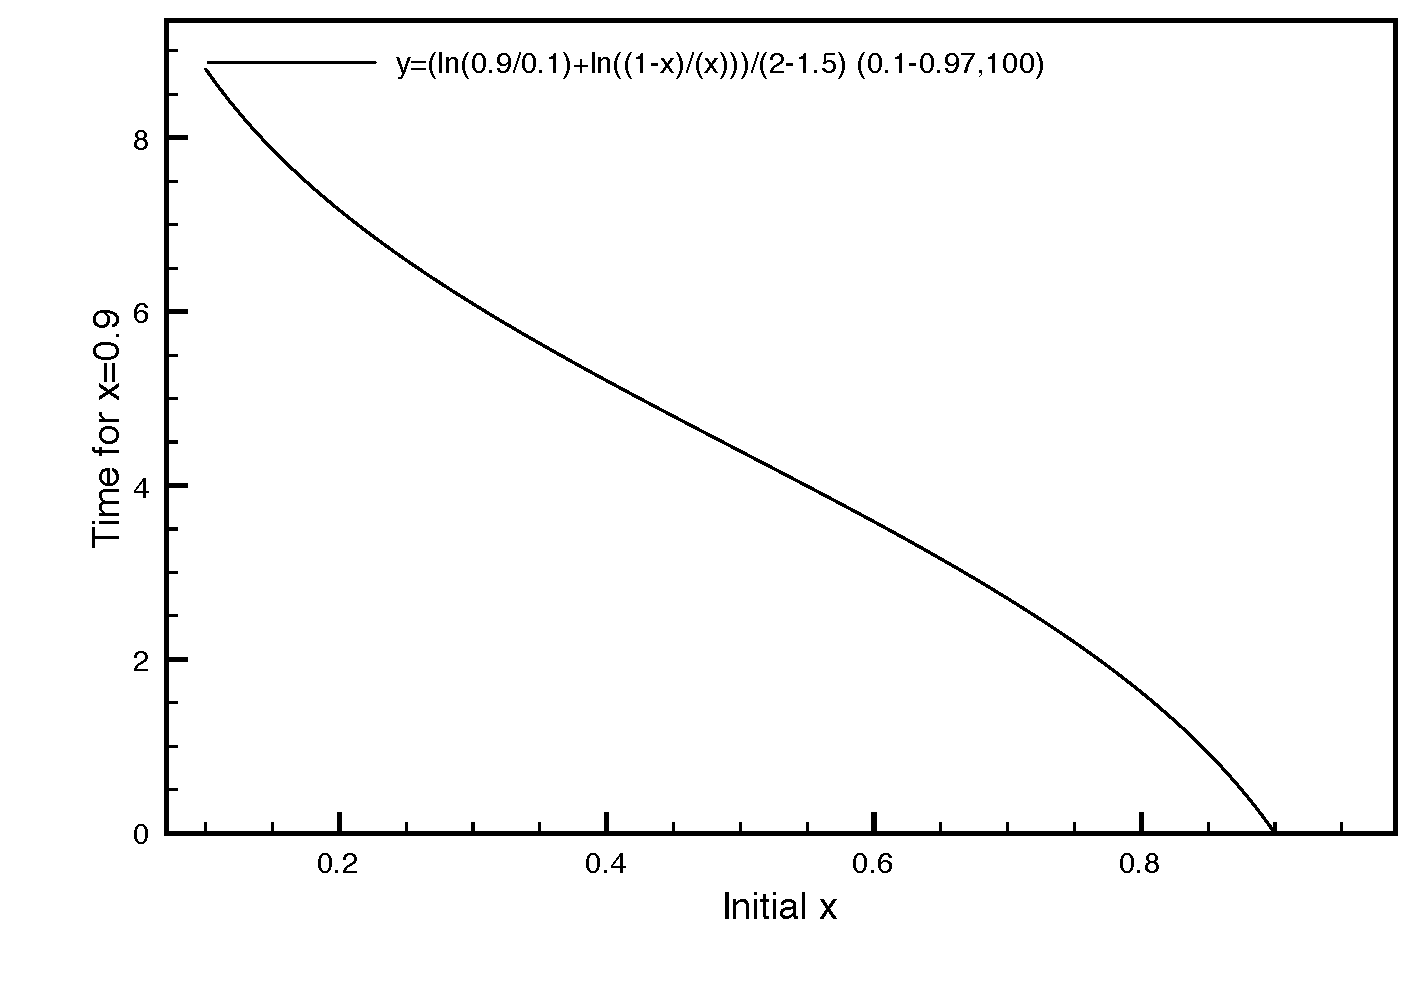
\includegraphics[width=7cm,height=7cm]{DominanceTimeVsInitialx.pdf}
    \else
      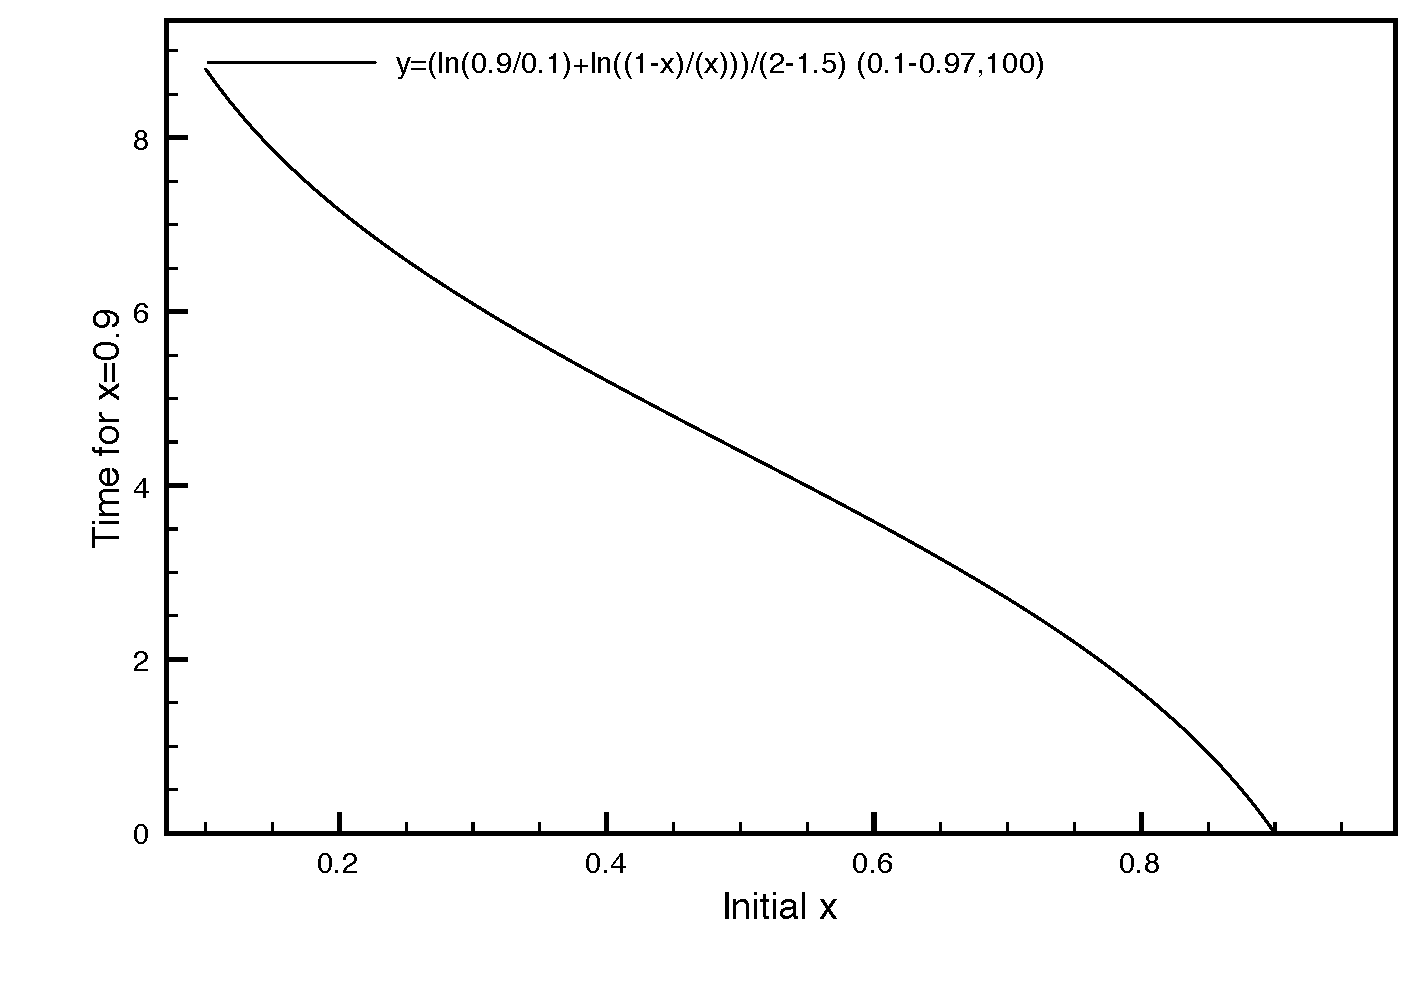
\includegraphics[width=7cm, height=7cm]{DominanceTimeVsInitialx.pdf}
    \fi
    \caption{Time when $x_{A}$ reach the $0.9$ fraction of population as a function of the initial $x_{A}$.}
    \label{FigAir2}
  \end{center}
\end{figure}

The problem with this model is that it does not let us  see the intrinsic process of selection, how each individual is chosen over the others for reproduction and finally a type invades the population. Later we will see the stochastic model for a situation of constant size and two types with different fitness.  
% ------------------------------------------------------------------------

%%% Local Variables: 
%%% mode: latex
%%% TeX-master: "../thesis"
%%% End: 
